\documentclass[a4paper]{article}
\usepackage{vntex}
%\usepackage[english,vietnam]{babel}
%\usepackage[utf8]{inputenc}

%\usepackage[utf8]{inputenc}
%\usepackage[francais]{babel}
\usepackage{a4wide,amssymb,epsfig,latexsym,multicol,array,hhline,fancyhdr}

\usepackage{tocbibind}
\usepackage{indentfirst}
\usepackage{float}
\usepackage{amsmath}
\usepackage{lastpage}
\usepackage[lined,boxed,commentsnumbered]{algorithm2e}
\usepackage{enumerate}
\usepackage{color}
\usepackage{graphicx}							% Standard graphics package
\usepackage{array}
\usepackage{tabularx, caption}
\usepackage{multirow}
\usepackage{multicol}
\usepackage{rotating}
\usepackage{graphics}
\usepackage{geometry}
\usepackage{setspace}
\usepackage{epsfig}
\usepackage{tikz}
\usetikzlibrary{arrows,snakes,backgrounds}
\usepackage{hyperref}
\hypersetup{urlcolor=blue,linkcolor=black,citecolor=black,colorlinks=true} 
%\usepackage{pstcol} 								% PSTricks with the standard color package

\newtheorem{theorem}{{\bf Định lý}}
\newtheorem{property}{{\bf Tính chất}}
\newtheorem{proposition}{{\bf Mệnh đề}}
\newtheorem{corollary}[proposition]{{\bf Hệ quả}}
\newtheorem{lemma}[proposition]{{\bf Bổ đề}}


%\usepackage{fancyhdr}
\setlength{\headheight}{40pt}
\pagestyle{fancy}
\fancyhead{} % clear all header fields
\fancyhead[L]{
 \begin{tabular}{rl}
    \begin{picture}(25,15)(0,0)
    \put(0,-8){
\includegraphics[width=8mm, height=8mm]{hcmut.png}}
    %\put(0,-8){\epsfig{width=10mm,figure=hcmut.eps}}
   \end{picture}&
	%
\includegraphics[width=8mm, height=8mm]{hcmut.png} & %
	\begin{tabular}{l}
		\textbf{\bf \ttfamily Trường Đại Học Bách Khoa Tp.Hồ Chí Minh}\\
		\textbf{\bf \ttfamily Khoa Khoa Học và Kỹ Thuật Máy Tính}
	\end{tabular} 	
 \end{tabular}
}
\fancyhead[R]{
	\begin{tabular}{l}
		\tiny \bf \\
		\tiny \bf 
	\end{tabular}  }
\fancyfoot{} % clear all footer fields
\fancyfoot[L]{\scriptsize \ttfamily Đồ án Thiết kế luận lý - Niên khóa 2019-2020}
\fancyfoot[R]{\scriptsize \ttfamily Trang {\thepage}/\pageref{LastPage}}
\renewcommand{\headrulewidth}{0.3pt}
\renewcommand{\footrulewidth}{0.3pt}


%%%
\setcounter{secnumdepth}{4}
\setcounter{tocdepth}{3}
\makeatletter
\newcounter {subsubsubsection}[subsubsection]
\renewcommand\thesubsubsubsection{\thesubsubsection .\@alph\c@subsubsubsection}
\newcommand\subsubsubsection{\@startsection{subsubsubsection}{4}{\z@}%
                                     {-3.25ex\@plus -1ex \@minus -.2ex}%
                                     {1.5ex \@plus .2ex}%
                                     {\normalfont\normalsize\bfseries}}
\newcommand*\l@subsubsubsection{\@dottedtocline{3}{10.0em}{4.1em}}
\newcommand*{\subsubsubsectionmark}[1]{}
\makeatother


\begin{document}

\begin{titlepage}
\begin{center}
ĐẠI HỌC QUỐC GIA THÀNH PHỐ HỒ CHÍ MINH \\
TRƯỜNG ĐẠI HỌC BÁCH KHOA \\
KHOA KHOA HỌC - KỸ THUẬT MÁY TÍNH 
\end{center}

\vspace{1cm}

\begin{figure}[h!]
\begin{center}

\includegraphics[width=3cm]{hcmut.png}
\end{center}
\end{figure}

\vspace{1cm}


\begin{center}
\begin{tabular}{c}
\multicolumn{1}{l}{\textbf{{\Large Đồ án Thiết kế luận lý}}}\\
~~\\
\hline
\\
\multicolumn{1}{l}{\textbf{{\Large Đề tài}}}\\
\\
\textbf{{\Huge Mô hình Đèn giao thông}}\\
\textbf{{\Huge có thể điều chỉnh}}\\
\\
\hline
\end{tabular}
\end{center}

\vspace{3cm}

\begin{table}[h]
\begin{tabular}{rrl}
\hspace{5 cm} & GVHD: & Phan Đình Thế Duy\\
& SV: & Nguyễn Trần Quang Minh - 1811083 \\
\end{tabular}
\end{table}

\begin{center}
{\footnotesize TP. HỒ CHÍ MINH, THÁNG 7/2020}
\end{center}
\end{titlepage}


%\thispagestyle{empty}
\newpage
\section*{Lời cam đoan}
Tôi xin cam đoan đây là nghiên cứu và thể hiện luận văn tốt nghiệp của bản thân thực hiện. Tôi không sao chép trái phép từ các đồ án – luận văn hay các tài liệu khác. Nếu những điều trên sai sự thật tôi xin chịu hoàn toàn trách nhiệm và mọi kỷ luật của khoa và nhà trường đề ra.
\begin{flushright}
TP. Hồ Chí Minh, tháng 7 năm 2020

	Nguyễn Trần Quang Minh
\end{flushright}


\newpage
\section*{Lời cảm ơn}
\addcontentsline{toc}{section}{Lời cảm ơn}
Tôi xin trân trọng gửi lời cảm ơn chân thành và tốt đẹp đến:

Thầy Phan Đình Thế Duy, người đã tận tình giúp đỡ, cung cấp tài liệu, thiết bị cần thiết và đưa ra những chỉ dẫn đúng đắn trong quá trình thực hiện đồ án.

Anh Nguyễn Ngọc Hanh, người đã hướng dẫn và hỗ trợ tôi phương pháp sử dụng hiệu quả các công cụ hiện có để thực hiện đồ án.

Bạn Trần Trọng Nguyên đã góp ý về phần thiết kế mạch, chọn lựa linh kiện và giúp tôi thực hiện đồ án một cách tốt nhất có thể.

Các thầy, cô trong bộ môn Kỹ thuật Máy tính, Khoa Khoa học và Kỹ thuật Máy tính đã tận tâm chỉ bảo và truyền thụ những kiến thức cho tôi trong suốt quá trình học từ trước đến nay.

Các anh, bạn cùng thực hiện Đồ án Thiết kế luận lý tại phòng thí nghiệm C6, những người đã tích cực hỗ trợ góp ý để tôi hoàn thiện môn học.

Cuối cùng, tôi rất biết ơn bố mẹ và anh chị đã chăm lo, cám ơn bạn bè đã ủng hộ tôi hoàn thành đồ án này.
\newpage
\section*{Tóm tắt đồ án}
\addcontentsline{toc}{section}{Tóm tắt đồ án}
Đề tài Đèn giao thông có thể điều chỉnh được hiện thực với mục đích mô phỏng lại hoạt động của tín hiệu giao thông tại một ngã tư. Khả năng điều chỉnh các mốc thời gian cũng như chuyển trạng thái tín hiệu là tính năng cơ bản nhất của một hệ thống đèn giao thông thông minh. Tuy vẫn còn thô sơ nhưng việc phát triển thêm các tính năng mới để đồ án này trở thành một hệ thống thông minh thực sự là hoàn toàn thực hiện được.

Quá trình hiện thực hoá đề tài bắt đầu từ việc liệt kê các trạng thái của đèn tín hiệu cùng với các chức năng bổ sung, qua đó lập nên một máy trạng thái đơn giản.

Đề tài này có sử dụng kit thí nghiệm BKIT PIC, 1 IC 74HC595 và 2 module điều khiển led 7 đoạn tích hợp với nhau để mô phỏng hoạt động của đèn giao thông qua các Led đỏ, xanh, vàng cùng với Led 7 đoạn hiển thị thời gian.

Đồ án này vẫn còn rất thô sơ do hạn chế phần nhiều về thời gian thực hiện cũng như giới hạn về tài chính.
\newpage
\tableofcontents
\newpage
\listoffigures
\newpage



%%%%%%%%%%%%%%%%%%%%%%%%%%%%%%%%%
\section{Giới thiệu đề tài}
\subsection{Tên đề tài:}

Hệ thống đèn giao thông có thể điều chỉnh được.

\subsection{Nhiệm vụ đề tài:}

Mô phỏng một hệ thống đèn giao thông tại một giao lộ, với khả năng điều chỉnh các thông số, trạng thái, và một số chức năng khác.

Hiện thực hệ thống trên một mô hình nhỏ.

\subsection{Ý nghĩa thực tiễn:}

Theo xu hướng chung,của thế giới, mọi hoạt động thường ngày đang dần được tự động hoá và trở nên "thông minh" hơn. Ở các nước tiên tiến, các hệ thống thông minh đã được áp dụng ngày một rộng rãi. Trong đó, hệ thống tín hiệu giao thông là một trong những ưu tiến phát triển hàng đầu của các nước này. Tín hiệu giao thông thông minh, cho phép điều chỉnh và có thể điều chỉnh tự động chính là chìa khoá để giải quyết ùn tắc giao thông, từ đó phát triển cơ sở hạ tầng cho các ngành kinh tế, logistics,....

\subsection{Cấu trúc báo cáo đồ án:}

Nội dung báo cáo được chia làm 3 phần như sau:

Phần 1: Giới thiệu đề tài

Phần 2: Cơ sở lý thuyết:

\begin{enumerate}
	\item Hoạt động cơ bản của hệ thống
	\item Phần cứng đã sử dụng
	\item Phần mềm đã sử dụng
	\item Máy trạng thái cho hệ thống
\end{enumerate}

Phần 3: Hiện thực và kết quả

\begin{enumerate}
	\item Hiện thực phần cứng
	\item Hiện thực phần mềm
	\item Mô phỏng hệ thống
	\item Kết luận
\end{enumerate}

\section{Hoạt động cơ bản của hệ thống:}
Tại một giao lộ thông thường, đèn tín hiệu sẽ có 4 trạng thái, (do hai trụ đèn đối diện nhau sẽ có cùng trạng thái), cụ thể như sau:

\begin{figure}[H]
\begin{center}
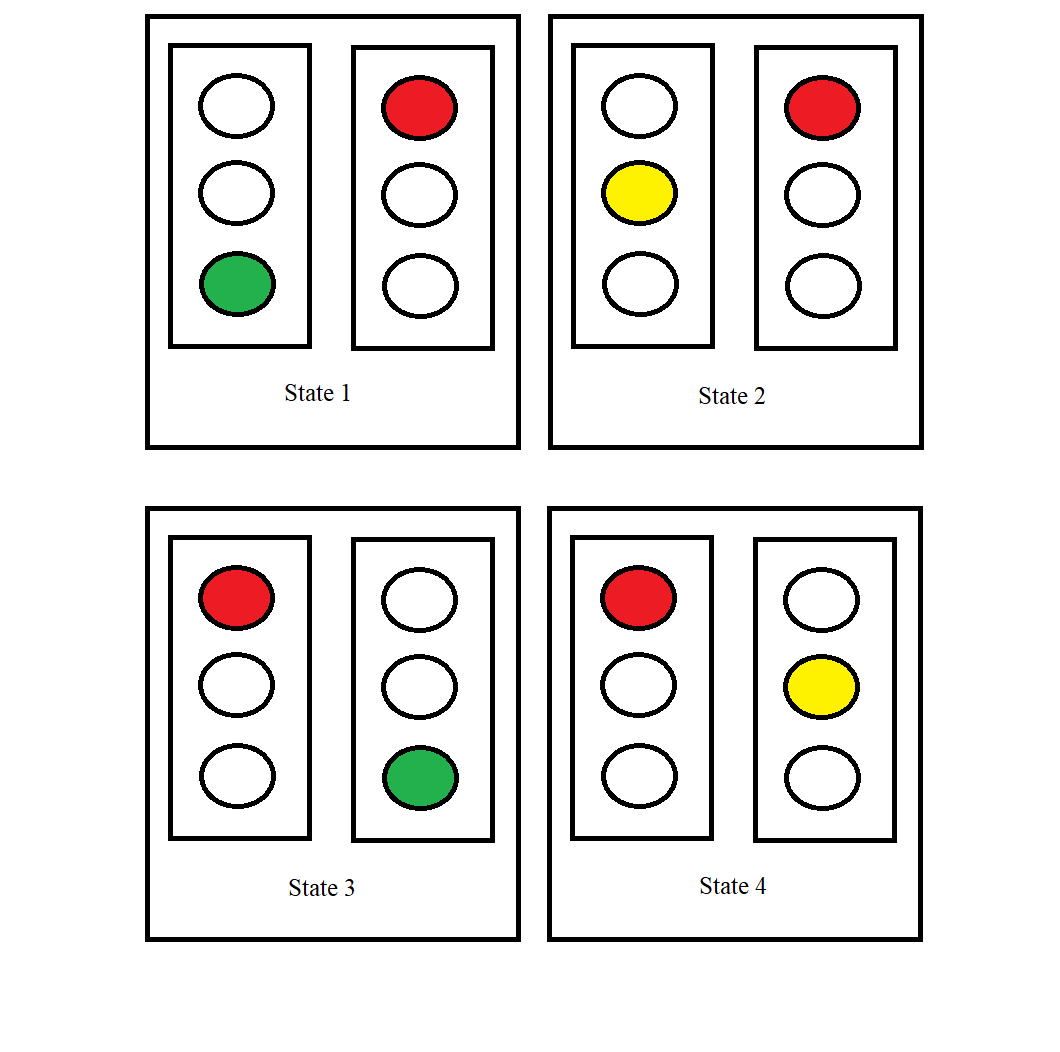
\includegraphics[width=12cm]{pic1.png}
\caption{Các trạng thái cơ bản}
\end{center}
\end{figure}

Bên cạnh đó, hệ thống sẽ tích hợp các chức năng khác như điều chỉnh thời gian của các đèn, chuyển trạng thái thủ công và trạng thái nhấp nháy đèn vàng. 

\section{Phần cứng đã sử dụng:}
\subsection{Kit thí nghiệm BKIT PIC:}
Bộ kit thí nghiệm BKIT PIC sử dụng chip PIC18F4620 của hãng Microchip. Đây là một vi điều khiển cung cấp hầu hết các ưu điểm của họ vi điều khiển PIC18 với các tính năng đặc biệt như công nghệ nanoWatt giúp tiết kiệm năng lượng, hỗ trợ nhiều mức xung.

Kit thí nghiệm được tích hợp các giao diện khác nhau, dễ dàng cho việc mở rộng thêm các thiết bị ngoại vi. Trên bộ kit này đã có sẵn ma trận nút nhấn, LCD và LED chỉ thị để thuận tiện cho việc lập trình và sửa lỗi. Một số chức năng cư bản đã được tích hợp sẵn bao gồm đồng hồ thời gian thực, ADC, PWM, UART,I2C, ....
\begin{figure}[H]
\begin{center}
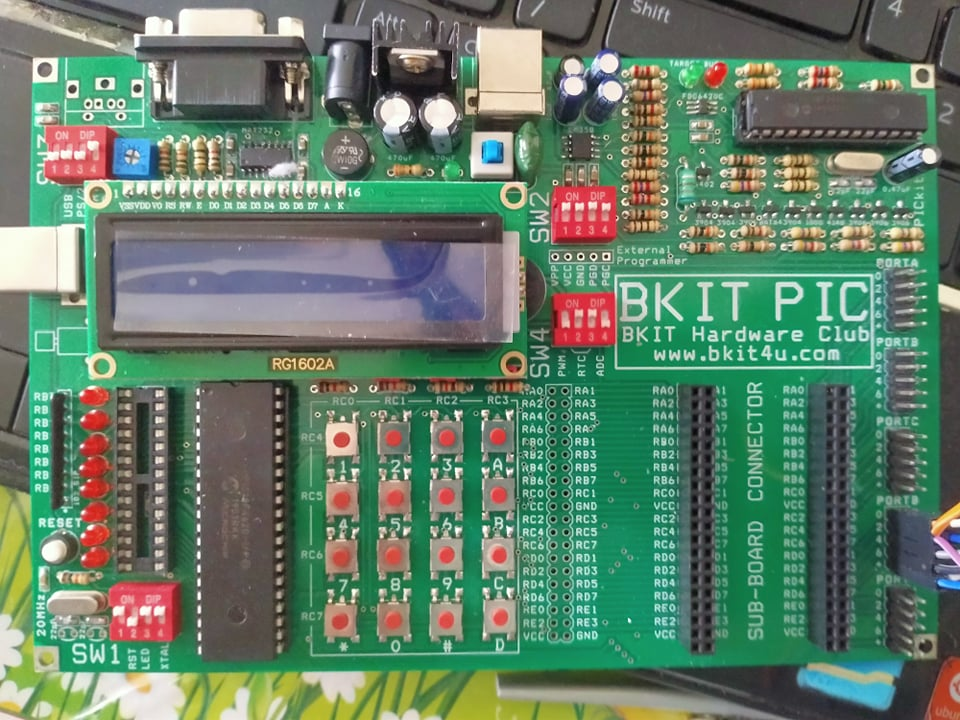
\includegraphics[width=12cm]{pic3.jpg}
\caption{Kit thí nghiệm BKIT PIC}
\end{center}
\end{figure}
\subsection{IC 74HC595N:}

Dùng để xuất ra 6 tín hiệu điều khiển các đèn giao thông.
\begin{figure}[H]
\begin{center}
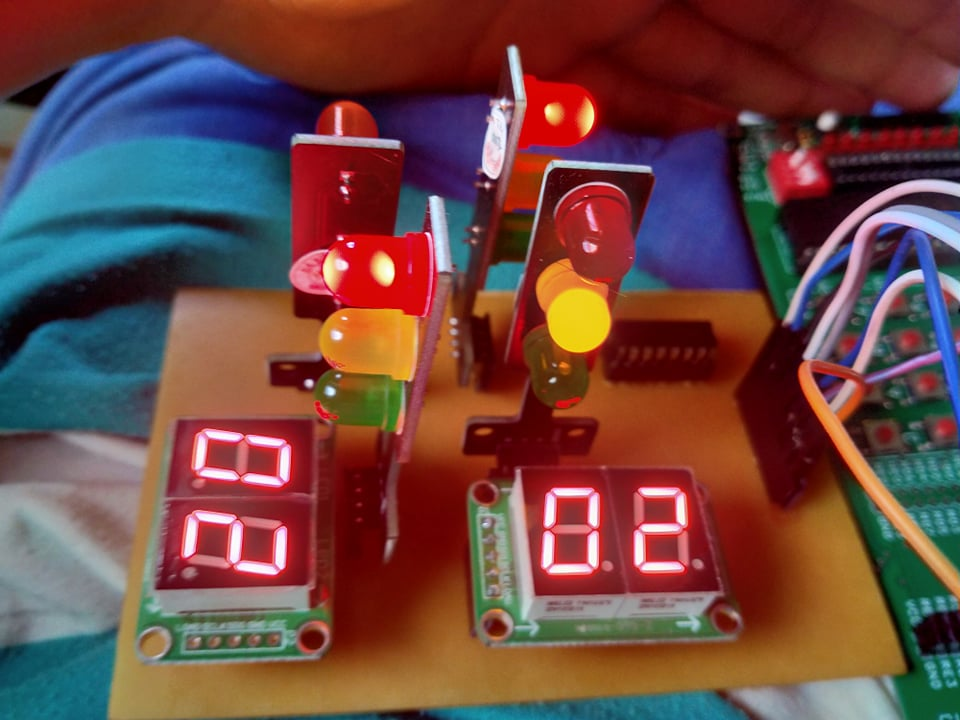
\includegraphics[width=5cm]{pic10.png}
\caption{74HC595N Pin Assignment}
\end{center}
\end{figure}

\subsection{Module Led 7 đoạn:}

Dùng để hiển thị thời gian chờ của đèn giao thông và được điều khiển bởi 2 IC 74HC595.
\begin{figure}[H]
\begin{center}
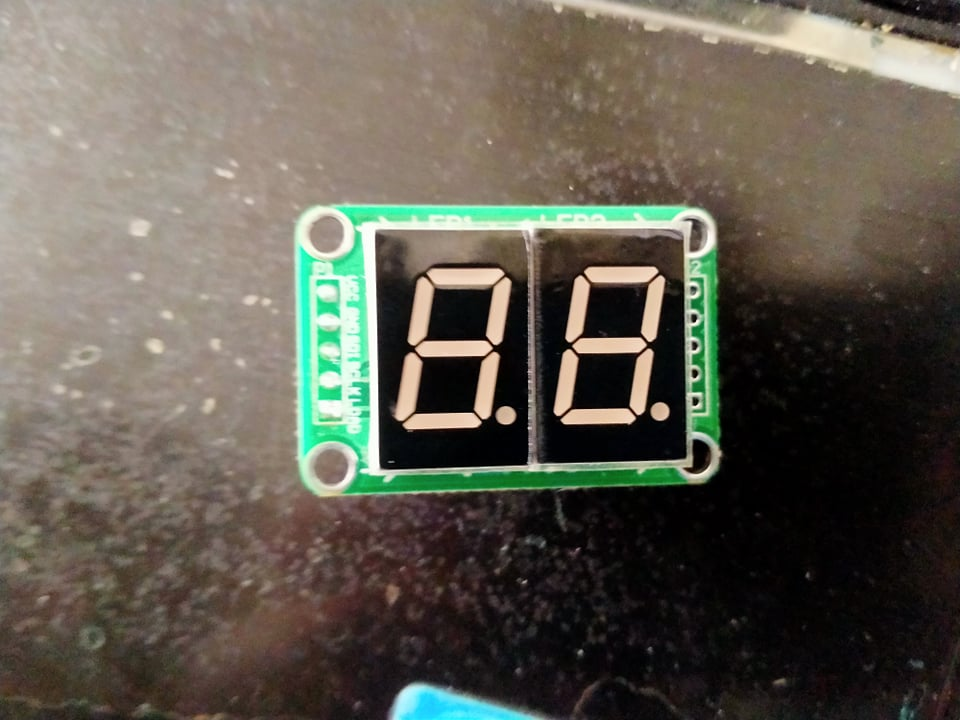
\includegraphics[width=5cm]{pic4.jpg}
\caption{Module led 7 đoạn}
\end{center}
\end{figure}

\subsection{Bộ 3 Led Đỏ - Xanh - Vàng}

Mô phỏng đèn tín hiệu giao thông.
 \begin{figure}[H]
\begin{center}
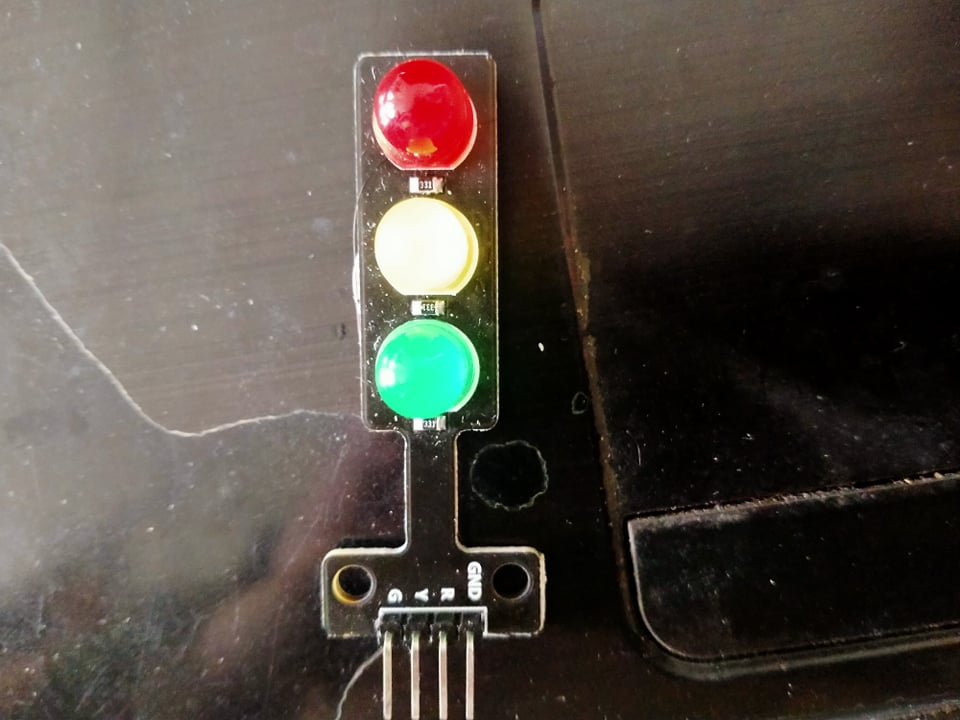
\includegraphics[width=5cm]{pic5.jpg}
\caption{Bộ 3 đèn Led}
\end{center}
\end{figure}
\subsection{Board mạch kết nối các module:}

In thủ công với các công cụ như bàn ủi, phíp đồng, máy khoan mài cầm tay.

Quá trình in mạch sử dụng các kiến thức, kỹ năng đã được học từ môn Thực tập phần cứng máy tính.
\begin{figure}[H]
\begin{center}
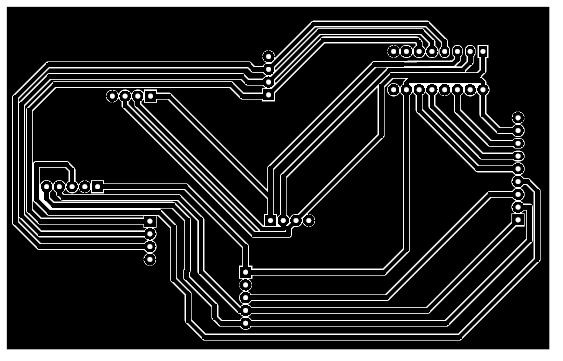
\includegraphics[width=12cm]{pic2.png}
\caption{Bản thiết kế mạch in}
\end{center}
\end{figure}
\section{Phần mềm đã sử dụng:}
\subsection{MPLAB X IDE:}
MPLAB X IDE là phần mềm hữu ích, được tích hợp các công cụ mạnh mẽ để lập trình, phát triển, sửa lỗi, hiệu chỉnh các thiết kế nhúng có sử dụng những dòng vi điều khiển của MIcrochip.

Phiên bản được sử dụng trong đồ án này là bản 3.26, là phiên bản rất ổn định cùng với trình biên dịch C18 v3.47
\subsection{Altium Designer:}
Altium designer là phần mềm PCB nổi tiếng bậc nhất hiện nay với nhiều tính năng đa dạng, các công cụ mạnh mẽ phục vụ cho việc thiết kế mạch in.

Phiên bản được sử dụng là bản 19.1.9 với giấy phép dành cho sinh viên được cung cấp bởi nhà phát hành Altium.

\section{Máy trạng thái cho hệ thống}
\begin{figure}[H]
\begin{center}
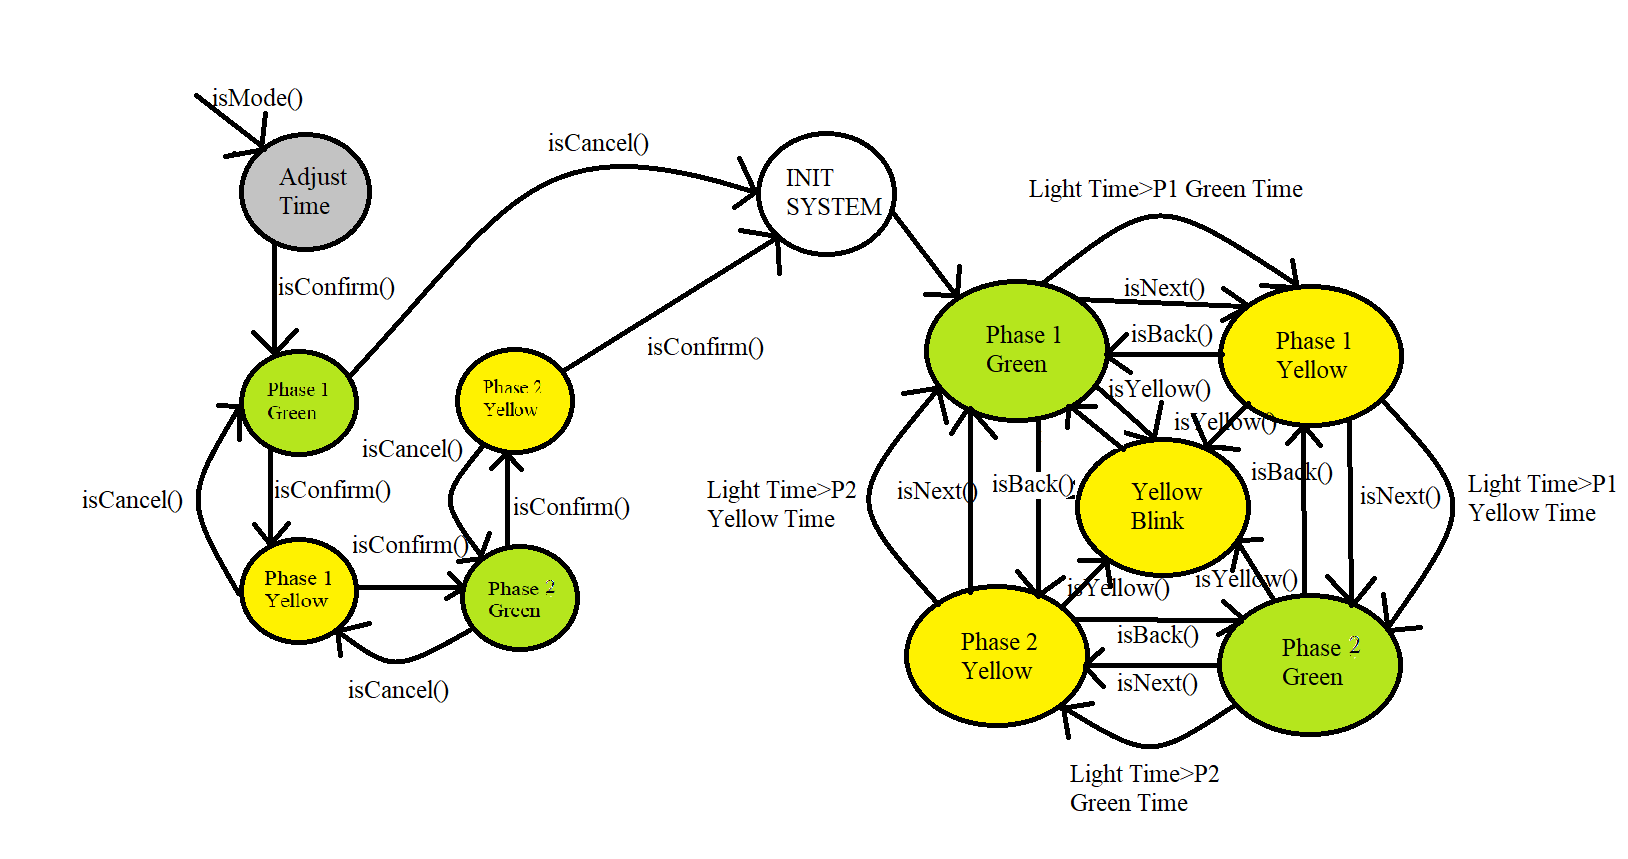
\includegraphics[width=17cm]{pic6.png}
\caption{Máy trạng thái của hệ thống}
\end{center}
\end{figure}

\section{Hiện thực phần cứng}
\subsection{Board mạch kết nối (mặt dưới)}
\begin{figure}[H]
\begin{center}
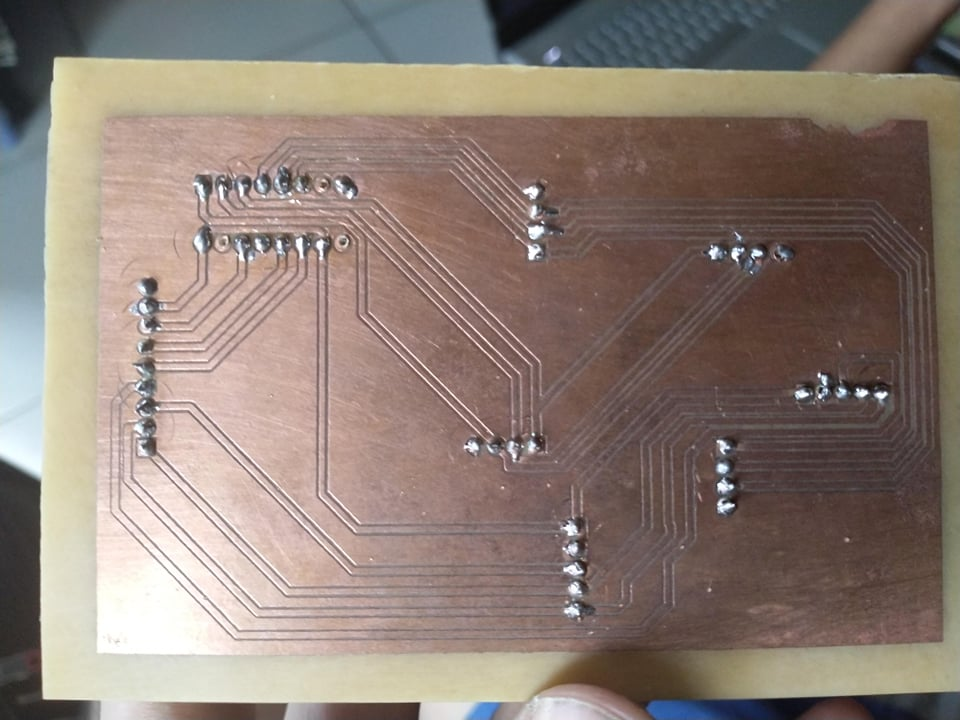
\includegraphics[width=14cm]{pic8.jpg}
\caption{Board mạch kết nối (mặt dưới)}
\end{center}
\end{figure}
\subsection{Board mạch kết nối (mặt trên)}
\begin{figure}[H]
\begin{center}

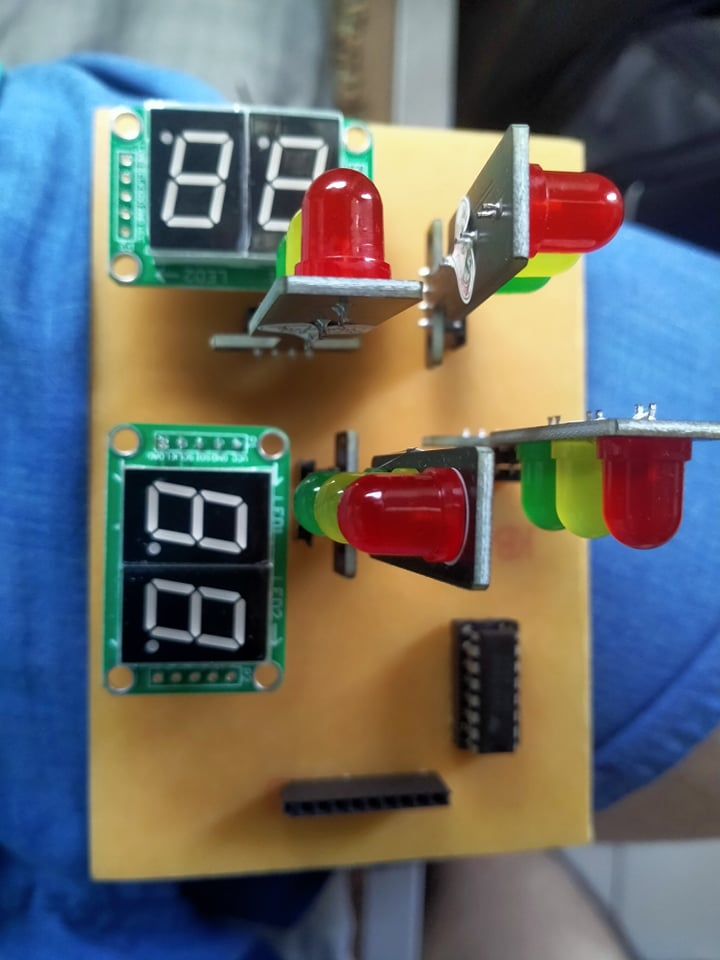
\includegraphics[width=10cm,angle=90]{pic7.jpg}
\caption{Board mạch kết nối (mặt trên)}
\end{center}
\end{figure}
\section{Hiện thực phần mềm}
\begin{figure}[H]
\begin{center}
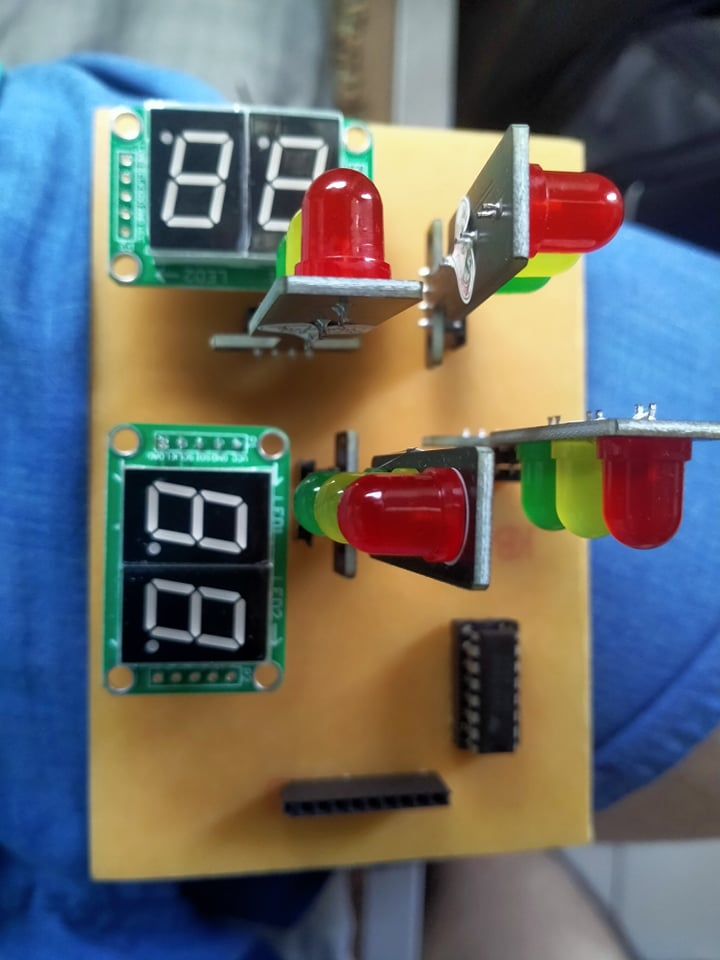
\includegraphics[width=12cm]{pic7.png}
\caption{Các hàm chính của chương trình}
\end{center}
\end{figure}
\section{Thử nghiệm hệ thống}

Khi hệ thống khởi động sẽ bắt đầu ngay vào trạng thái chạy tự động, tức là đèn sẽ tự chuyển pha theo thời gian đính sẵn.

Khi người dùng cần điều chỉnh thời gian theo ý muốn, nhấn phím * trên bàn phím, hế thống sẽ vào trạng thái nhận dữ liệu lần lượt là thười gian của mỗi pha (4 oha tất cả). Lúc này, thời gian có thể được điều chỉnh tăng (phím 2) hay giảm (phím 8). Xác nhận thời gian bằng cách nhấn phím 5. Khi cần trở lại trạng thái trước để điều chỉnh thời gian của pha trước đó hoặc thoát chế độ chỉnh sửa, nhấn phím \#.

Ở trạng thái chạy tự động, nếu người dùng có nhu cầu chuyển pha lập tức thì có thể nhấn phím 6 (pha tiếp theo) hoặc phím 4 (pha trước đó). Ngoài ra, người dùng có thể đặt chế độ chuyển pha thủ công hoàn toàn nếu nhấn phím B. Tại chế độ này, việc chuyển pha chỉ dựa vào phím 4 và phím 6. Chuyển về chế độ tự động nếu nhấn lại phím B

Khi cần chuyển sang trạng thái LED vàng nhấp nháy, người dùng có thể nhấn phím C và cũng nhấn phím này khi cần trở lại chế độ tự động.


\subsection{Trạng thái Phase 1 Green}
\begin{figure}[H]
\begin{center}
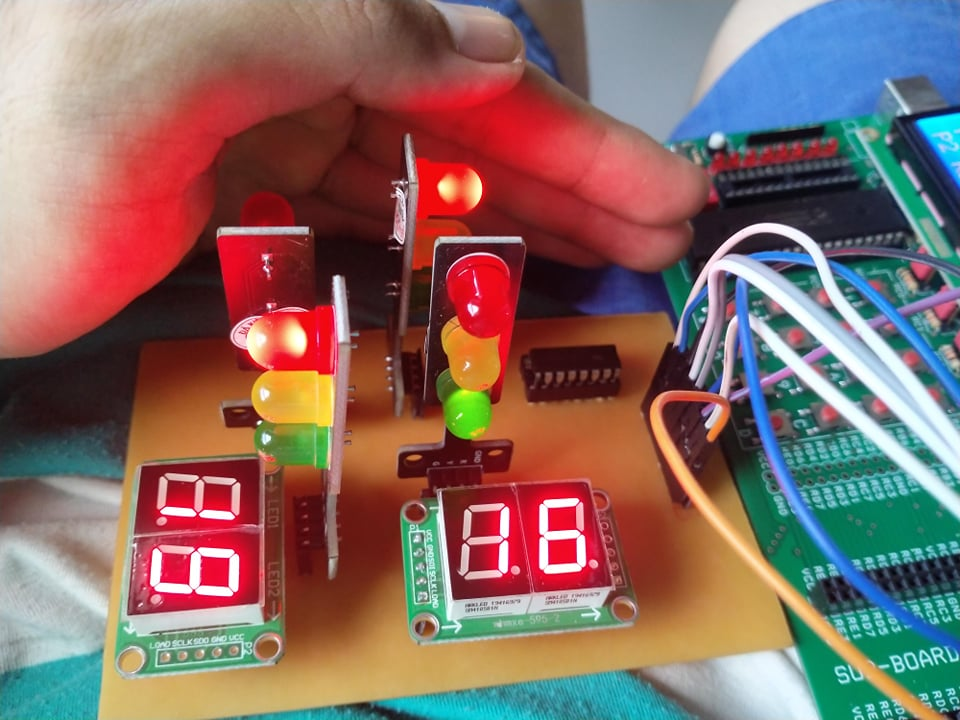
\includegraphics[width=12cm]{pic9.jpg}
\caption{Trạng thái Phase 1 Green}
\end{center}
\end{figure}
\subsection{Trạng thái Phase 1 Yellow}
\begin{figure}[H]
\begin{center}
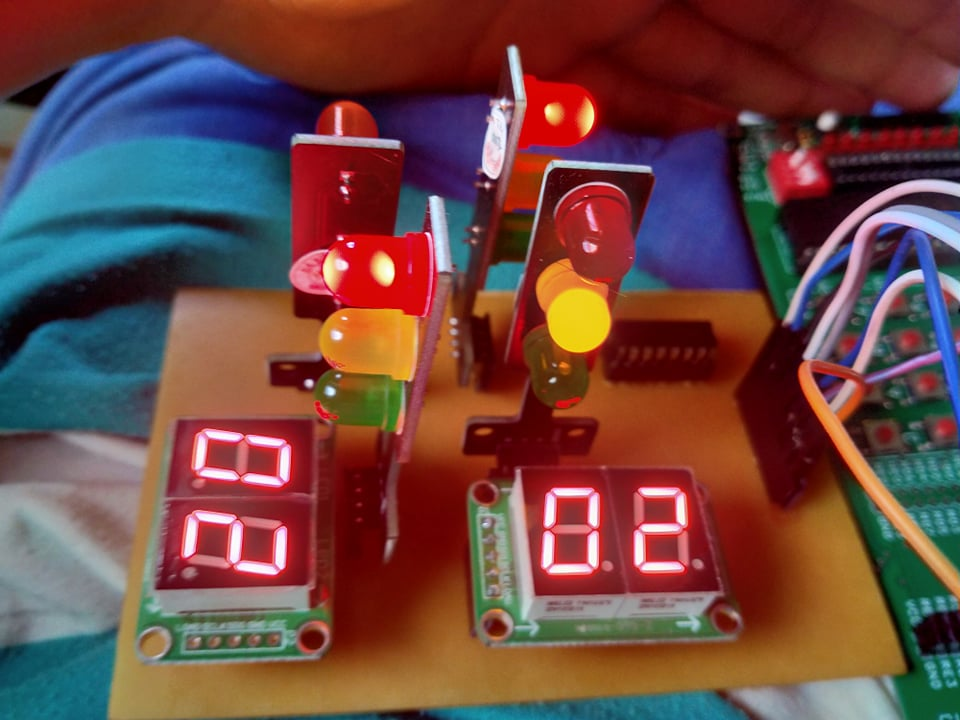
\includegraphics[width=12cm]{pic10.jpg}
\caption{Trạng thái Phase 1 Yellow}
\end{center}
\end{figure}
\subsection{Trạng thái Phase 2 Green}
\begin{figure}[H]
\begin{center}
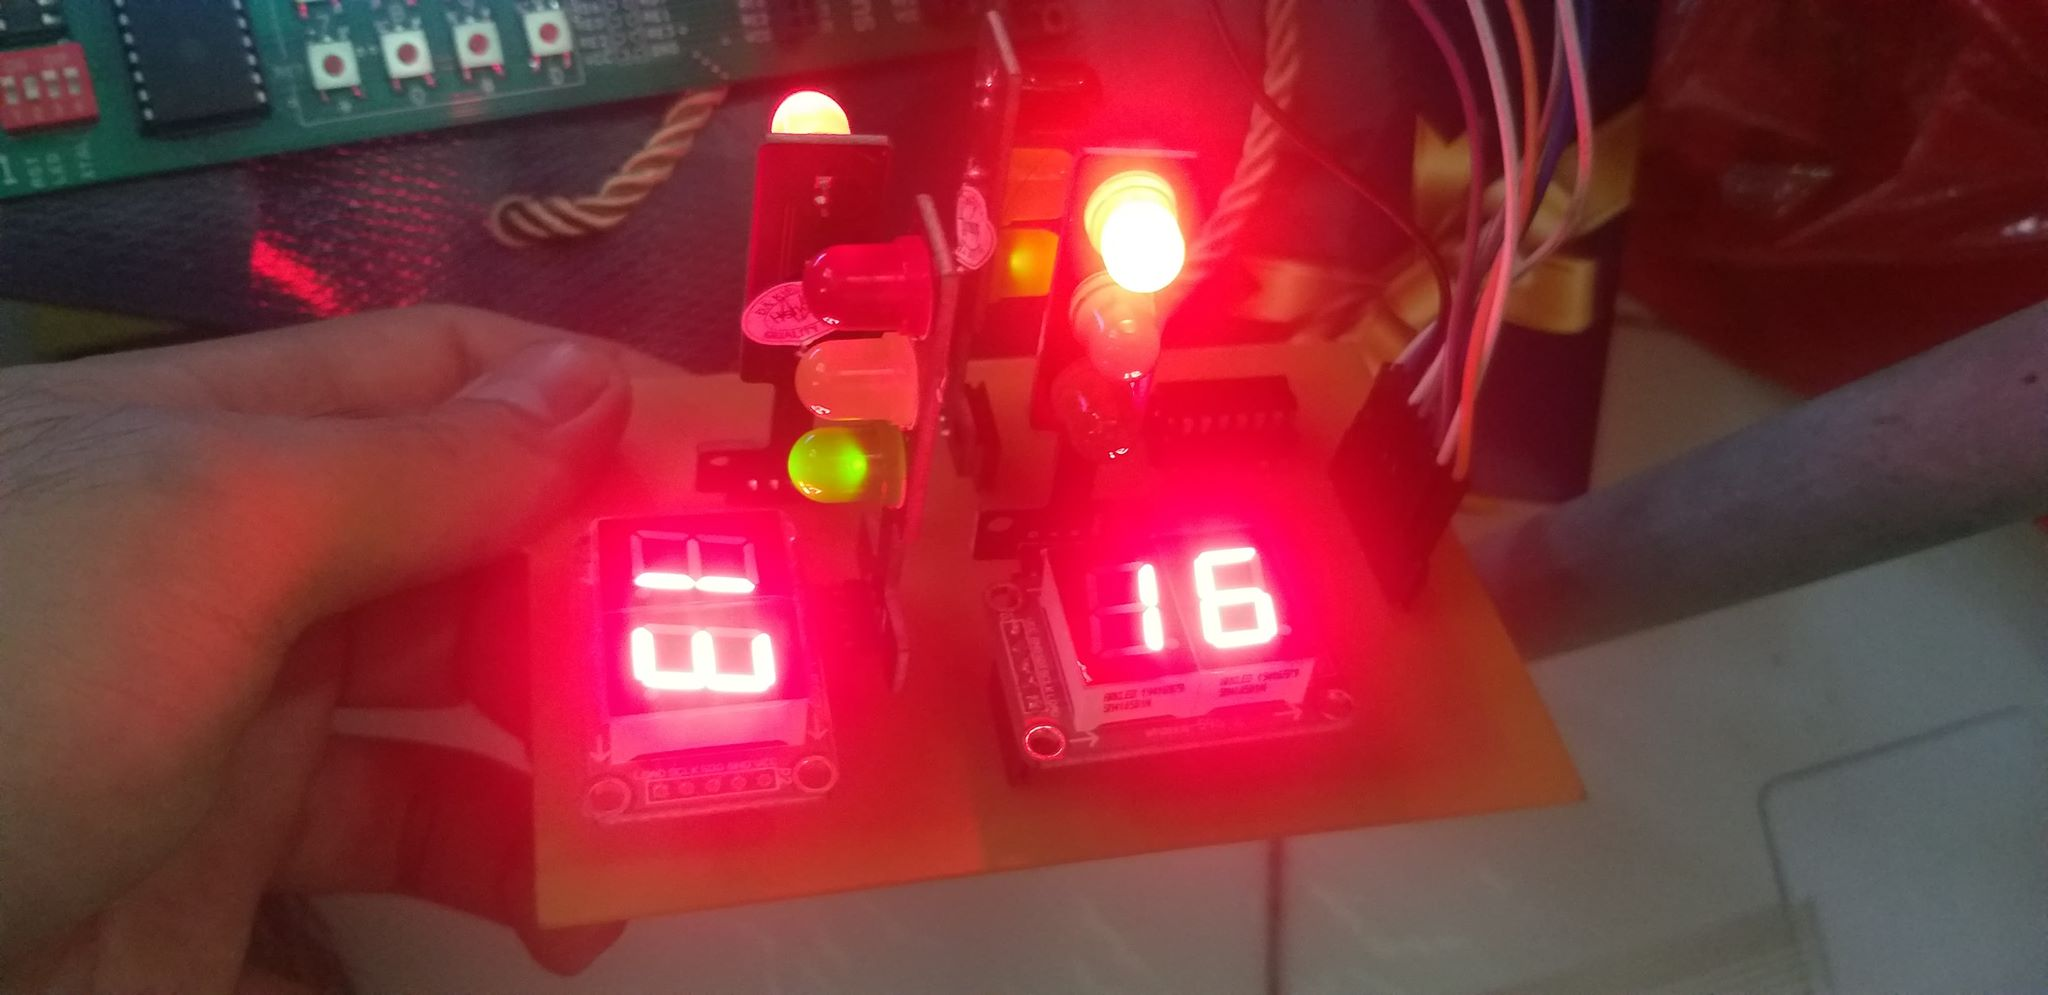
\includegraphics[width=12cm]{pic11.jpg}
\caption{Trạng thái Phase 2 Green}
\end{center}
\end{figure}
\subsection{Trạng thái Phase 2 Yellow}
\begin{figure}[H]
\begin{center}
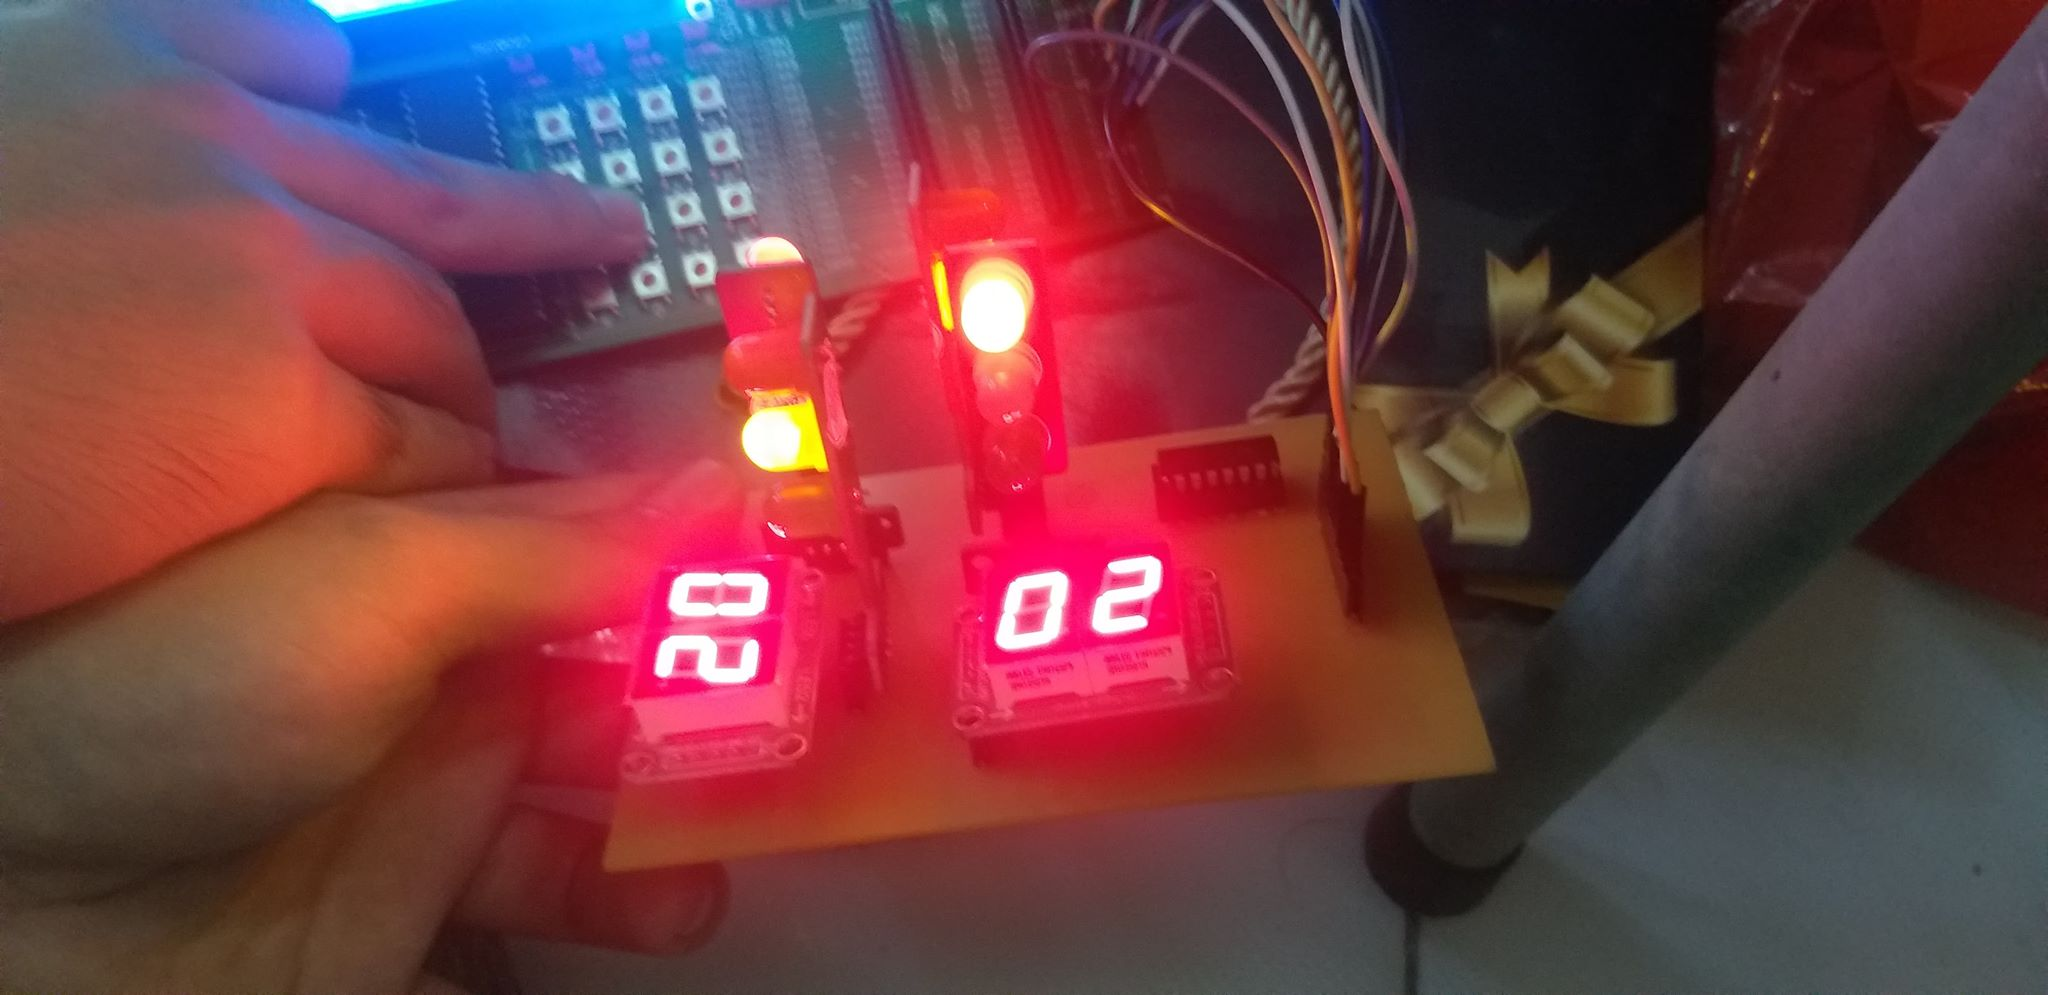
\includegraphics[width=12cm]{pic12.jpg}
\caption{Trạng thái Phase 2 Yellow}
\end{center}
\end{figure}
\subsection{Trạng thái Yellow Blink}
\begin{figure}[H]
\begin{center}
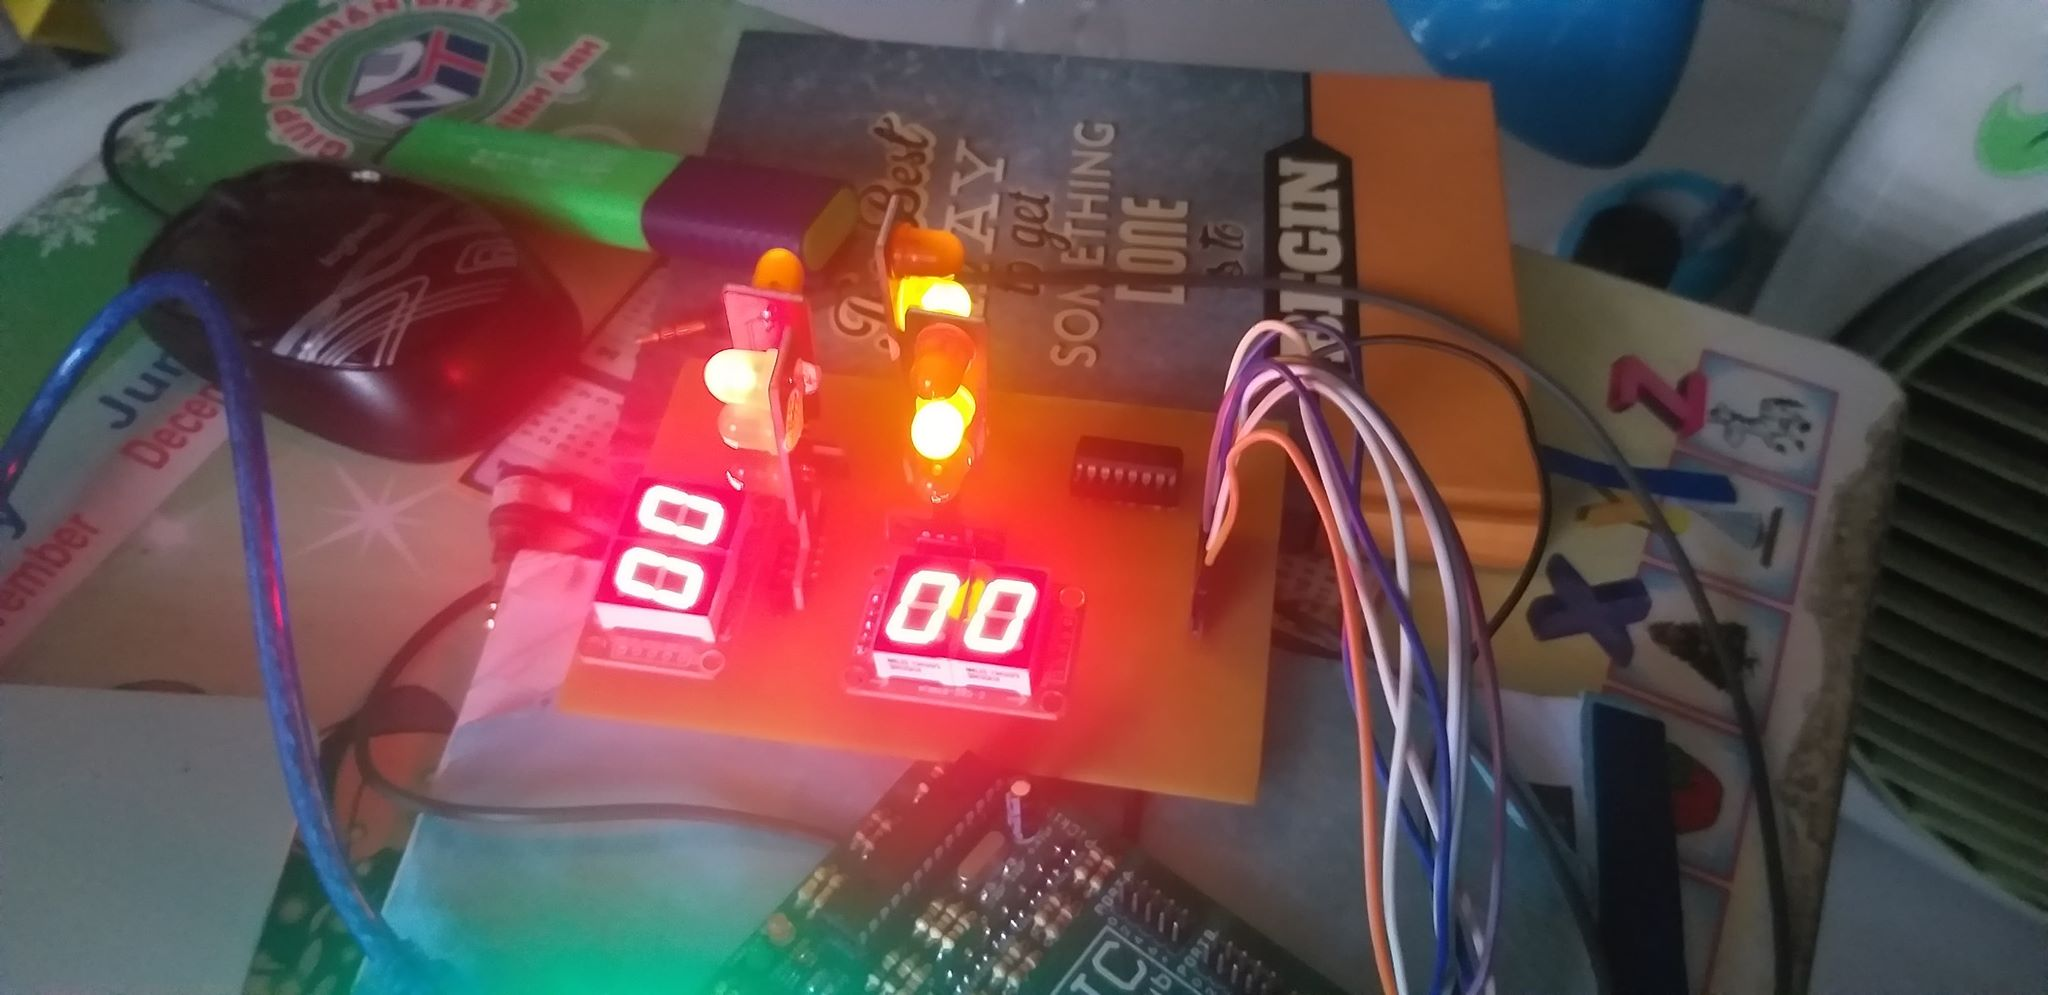
\includegraphics[width=12cm]{pic13.jpg}
\caption{Trạng thái Yellow Blink}
\end{center}
\end{figure}
\subsection{Trạng thái chỉnh sửa thời gian}
\begin{figure}[H]
\begin{center}
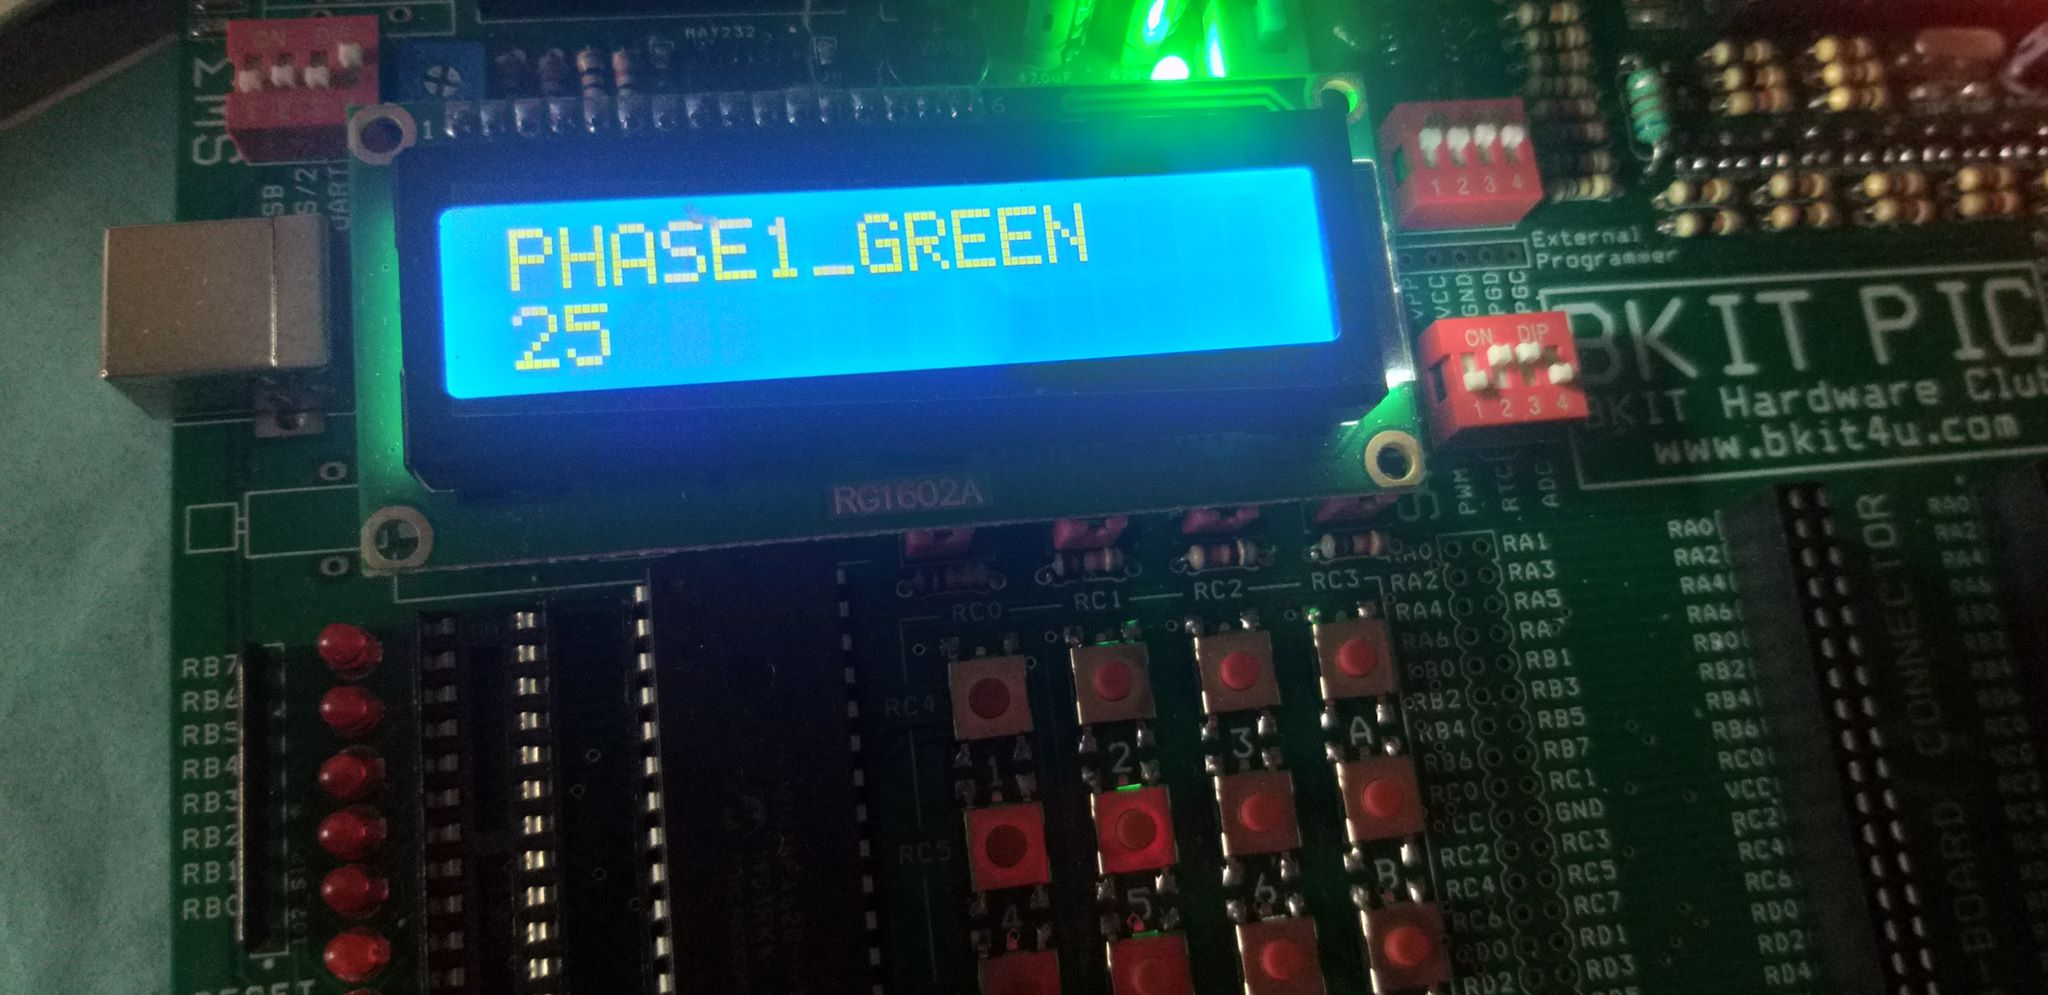
\includegraphics[width=12cm]{pic14.jpg}
\caption{Chỉnh thời gian cho Phase 1 Green}
\end{center}
\end{figure}

%%%%%%%%%%%%%%%%%%%%%%%%%%%%%%%%%
\section{Kết luận}
\subsection{Kết quả đạt được:}

Từ đề tài xây dựng hệ thống đèn giao thông có thể điều chỉnh, sản phẩm được hoàn thiện là một mô hình nút giao thông nhỏ với các chức năng chính sau:

\begin{enumerate}
	\item Chuyển trạng thái khi hết thời gian mỗi pha.
	\item Chuyển trạng thái theo lệnh của người điều khiển.
	\item Thay đổi mốc thời gian các pha.
	\item Nhấp nháy đèn vàng liên tục.
\end{enumerate}

\subsection{Quá trình thực hiện đề tài:}
Trải qua 2 tháng nghiên cứu và thực hiện đề tài, tôi đã gặp không ít khó khăn như tìm mua linh kiện, in mạch, hạn chế về thời gian, .... Nhưng nhờ sự hỗ trợ tích cực từ thầy Phan Đình Thế Duy và các anh, các bạn ở lớp Đồ án phòng thí nghiệm C6, sản phẩm cuối cùng đã được hoàn thiện.

\subsection{Mở rộng và phát triển đề tài:}
\subsubsection{Tích hợp camera:}
Ở đề tài này chỉ dừng lại ở việc tạo ra một hệ thống có thể điều chỉnh. Một hướng phát triển mới có thể được cân chính là tích hợp camera an ninh để cso thể nhận dạng lưu lượng xe hiện tại, ghi nhận lại, từ đó đưa ra thời gian chờ đèn tín hiệu thích hợp nhằm giảm tránh tối thiểu ùn tắc giao thông.
\subsubsection{Mở rộng thêm nhiều nút giao thông:}
Không chỉ dừng lại ở việc diều chỉnh tín hiệu một cách tự động cho một nút giao thông, giờ đây ta có thể mở rộng ra thành một mạng lưới với quy mô lớn hơn.
Việc phối hợp đèn tín hiệu giao thông ở các nút giao thông khác nhau là một bài toán rất khó khăn và vẫn đang được nghiên cứu. 

Mở rộng đề tài theo hướng đi này sẽ cần kết hợp rất nhiều kiến thức đa ngành như toán học, giao thông, xây dựng ,...
%%%%%%%%%%%%%%%%%%%%%%%%%%%%%%%%%
\begin{thebibliography}{80}


\bibitem{comnet}
BKIT Hardware Club, \textit{MPLAB 8.36 và MPLAB C18 trên BKIT PIC}
\bibitem{ttpc}
Bộ môn KTMT - Khoa học \& KTMT, trường Đại học Bách Khoa TP.HCM, \textit{Thực tập phần cứng máy tính}

\bibitem{dta}
 ON Semiconductor, “8-Bit Serial-Input/Serial or. Parallel-Output Shift. Register with Latched. 3-State Outputs” 74HC595 datasheet, March 2000.
\bibitem{dta2}
 Microchip, “28/40/44-Pin Enhanced Flash Microcontrollers with 10-Bit A/D and nanoWatt Technology” PIC18F2525/2620/4525/4620 Data Sheet, February 2008.

\end{thebibliography}
\end{document}

